\section{Baseline Visual Acuity Analysis}

\subsection{Distribution of Treatment-Naïve Visual Acuity}

To establish a realistic initialization model for our simulations, we analyzed baseline (treatment-naïve) visual acuity measurements from 2,029 patients in our database. Understanding the true distribution of starting visual acuities is critical for developing accurate simulation models that reflect real-world patient populations.

\begin{figure}[h]
    \centering
    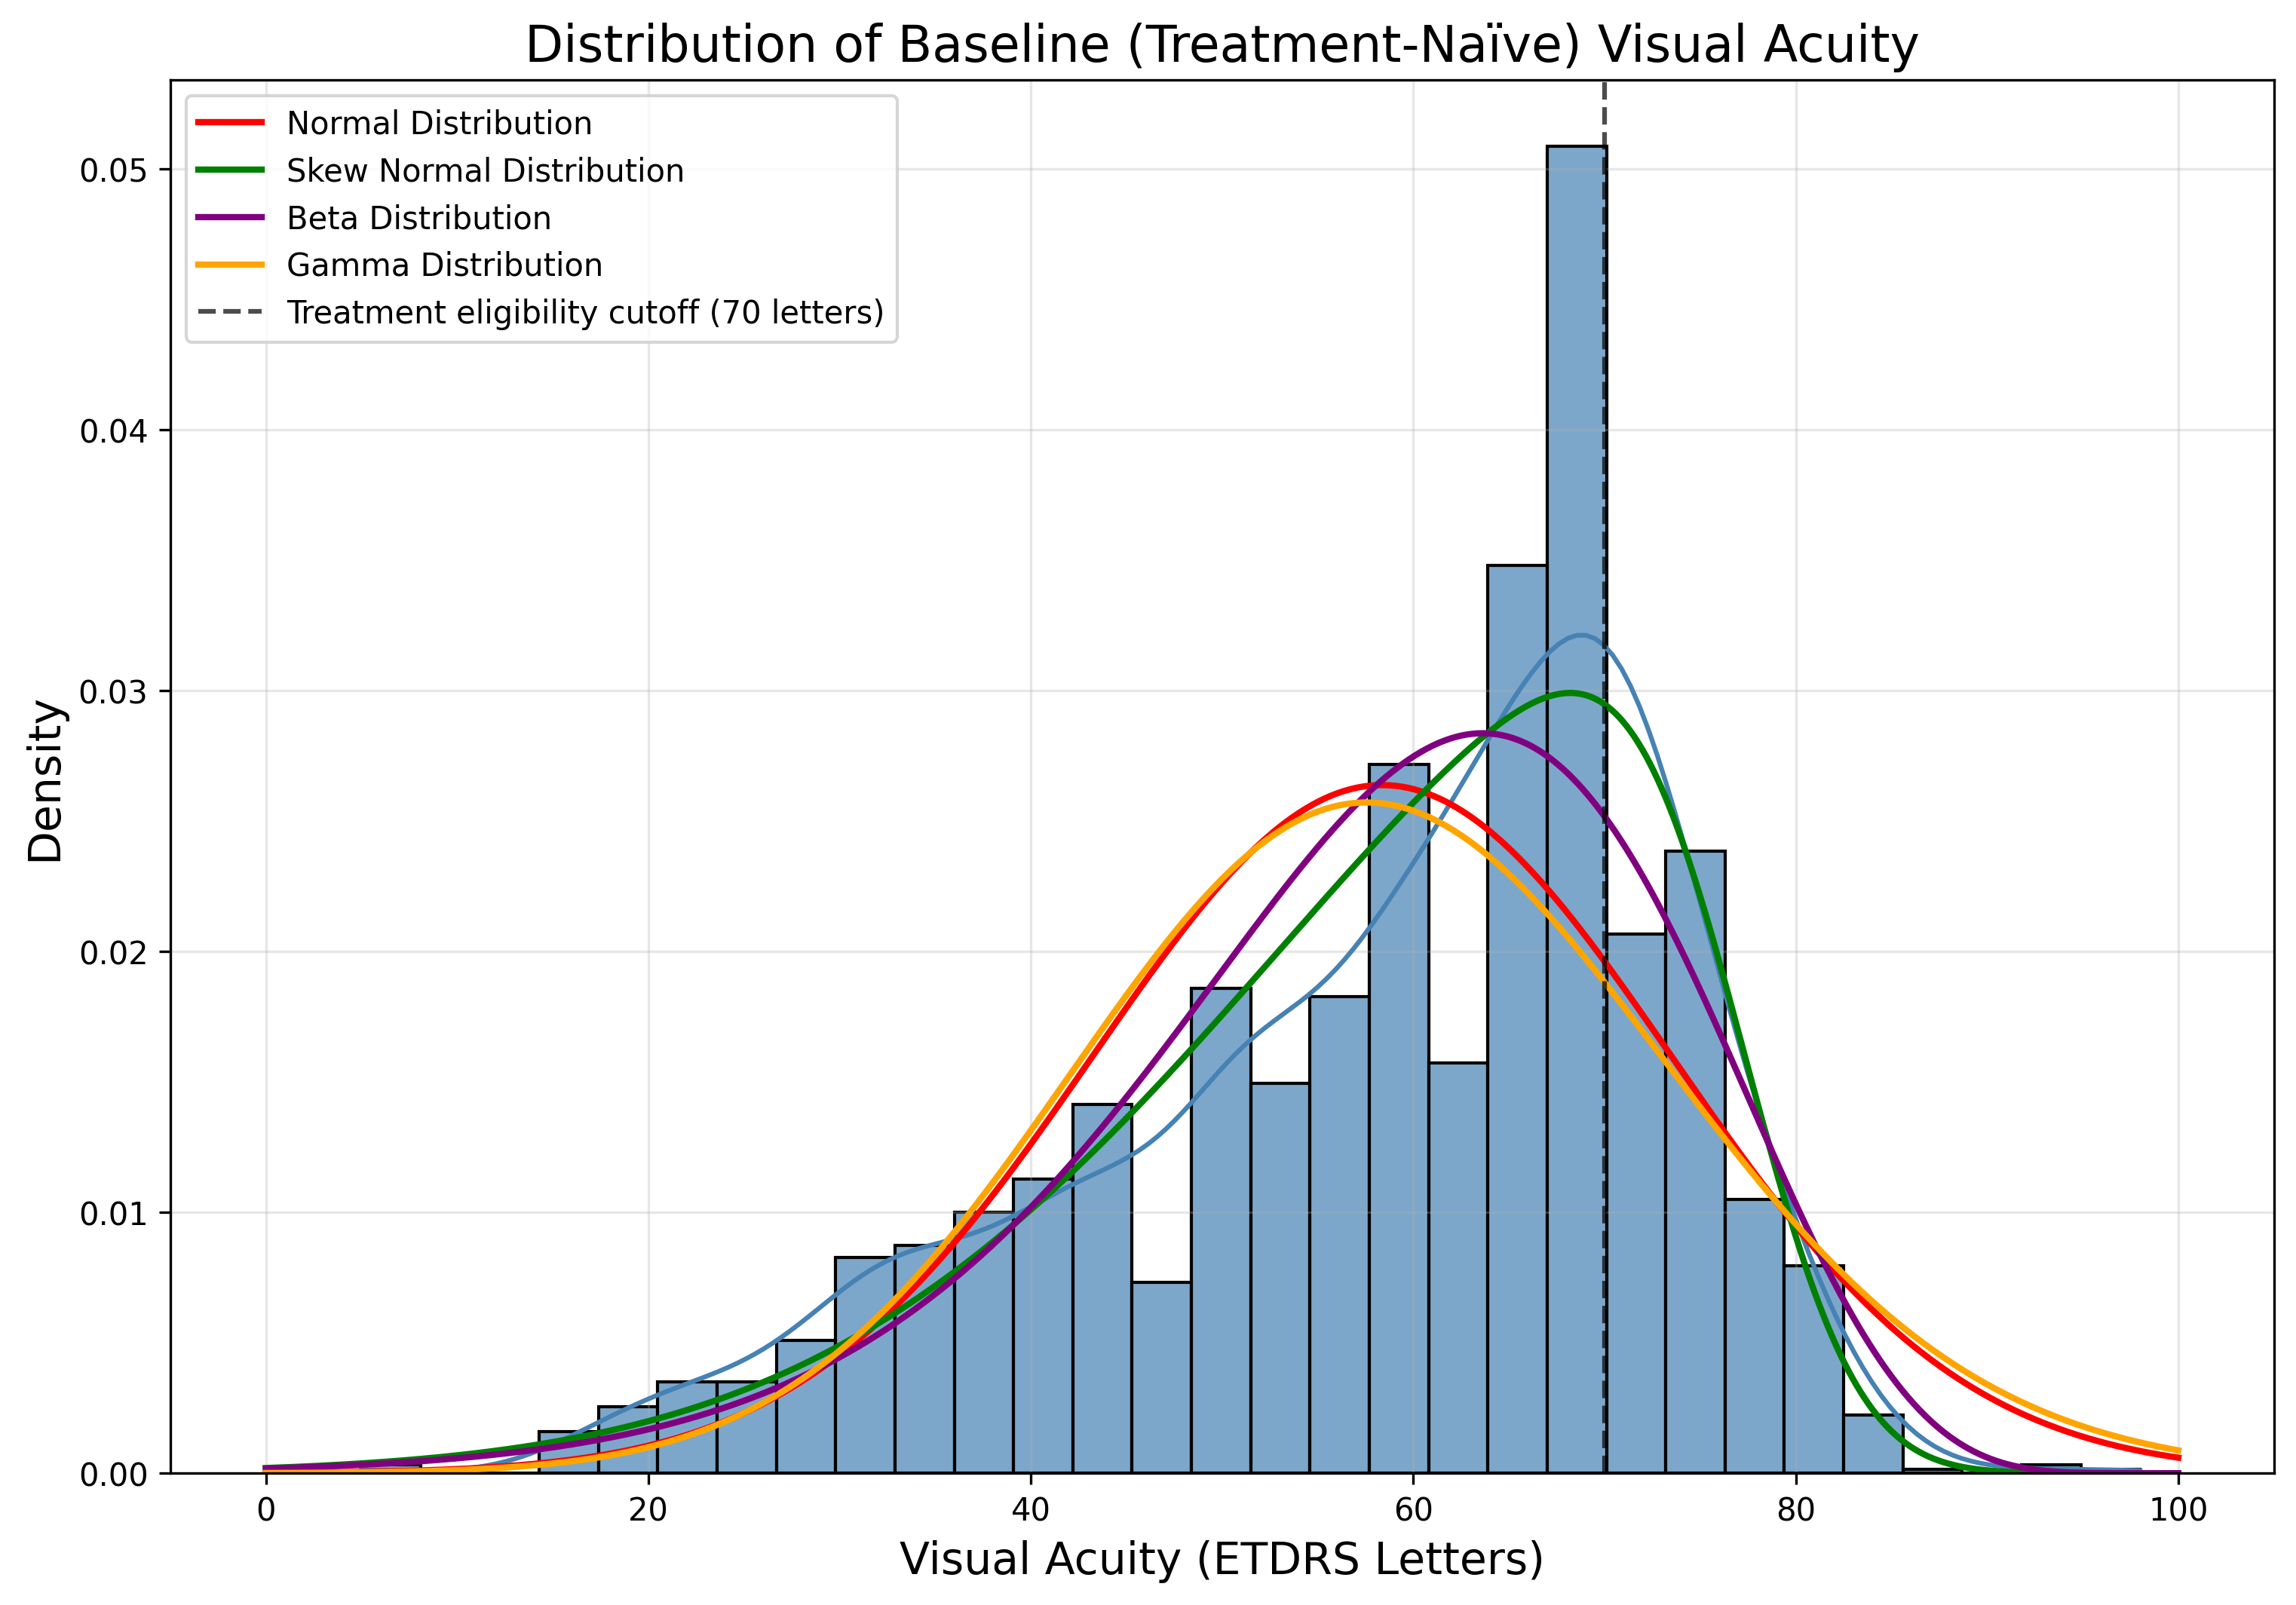
\includegraphics[width=0.9\textwidth]{figures/acuity/baseline_va_distribution.png}
    \caption{Distribution of baseline (treatment-naïve) visual acuity with fitted probability distributions. The dashed vertical line represents the treatment eligibility cutoff at 70 ETDRS letters.}
    \label{fig:baseline_va_distribution}
\end{figure}

\subsection{Key Statistical Findings}

Our analysis revealed several important characteristics of the baseline visual acuity distribution:

\begin{itemize}
    \item \textbf{Central Tendency}: The mean baseline VA was 58.36 ETDRS letters (approximately 20/63 Snellen equivalent), with a median of 62.00 letters.
    \item \textbf{Dispersion}: The standard deviation was 15.12 letters, indicating substantial variability in baseline vision.
    \item \textbf{Shape Characteristics}: The distribution exhibited negative skewness (-0.72) and slight platykurtosis (-0.14), indicating more patients with lower vision than would be expected in a normal distribution.
    \item \textbf{Range}: Baseline VA ranged from 5.0 to 98.0 letters, with 95\% of patients falling between 29.0 and 78.0 letters.
\end{itemize}

When fitted to standard probability distributions, the Beta distribution provided the best fit (lowest AIC score), capturing the non-normal characteristics of the data. This finding is important as many simulation models incorrectly assume normally distributed baseline visual acuities.

\subsection{Visual Acuity Stratification}

We stratified patients by baseline visual acuity ranges to better understand the clinical composition of our population:

\begin{table}[h]
\centering
\caption{Distribution of patients by baseline visual acuity ranges}
\label{tab:va_stratification}
\begin{tabular}{lrr}
\hline
\textbf{Visual Acuity Range} & \textbf{Patient Count} & \textbf{Percentage} \\
\hline
Very Poor (0-30 letters) & 118 & 5.8\% \\
Poor (31-50 letters) & 451 & 22.2\% \\
Moderate (51-70 letters) & 1,046 & 51.6\% \\
Good (71-85 letters) & 410 & 20.2\% \\
Excellent (86-100 letters) & 4 & 0.2\% \\
\hline
\end{tabular}
\end{table}

Notably, 51.6\% of patients fell within the moderate VA range (51-70 letters), aligning with the typical treatment eligibility criteria for anti-VEGF therapy in wet AMD. The small proportion of patients with excellent vision (0.2\%) confirms the rarity of preserved vision in treatment-naïve wet AMD.

\subsection{Treatment Eligibility Threshold Effect}

The analysis confirmed the impact of the 70-letter treatment eligibility threshold, with clear distributional effects:

\begin{itemize}
    \item Only 20.4\% of patients had baseline VA above 70 letters
    \item The 75th percentile of the distribution was exactly at the 70-letter threshold
    \item The distribution shows a notable peak just below the threshold (65-69 letters)
\end{itemize}

Further investigation of patients with VA $>$ 70 letters revealed that 57.7\% showed vision decline at their second visit, with a mean decline of 4.52 letters. This suggests that many patients with good initial VA were experiencing active disease progression that warranted treatment despite being above the standard eligibility threshold.

\subsection{Percentile Analysis}

To provide precise reference points for our simulation model, we calculated key percentiles of the baseline VA distribution:

\begin{itemize}
    \item 5th percentile: 29.0 letters
    \item 10th percentile: 35.0 letters
    \item 25th percentile: 50.0 letters
    \item 50th percentile: 62.0 letters
    \item 75th percentile: 70.0 letters
    \item 90th percentile: 75.0 letters
    \item 95th percentile: 78.0 letters
\end{itemize}

This percentile analysis provides evidence-based boundaries for ceiling and floor effects in vision improvement models, with the 95th percentile (78 letters) supporting our simulation model's ceiling of 85 letters as an appropriate upper bound.

\subsection{Implications for Vision Change Models}

Based on this analysis, we identified several key modifications needed for our simulation's vision change models:

\begin{enumerate}
    \item \textbf{Baseline Distribution}: Initial visual acuity should be modeled using a Beta distribution rather than the previously used normal distribution, with parameters derived from our observed data.
    
    \item \textbf{Segmented Response Profiles}: Treatment response should be segmented based on baseline VA, with differential improvement potential reflecting the ceiling effects observed in patients with better starting vision.
    
    \item \textbf{Vision Fluctuation}: The substantial variability observed (SD = 15.12 letters) justifies implementing realistic vision fluctuations in our model.
    
    \item \textbf{Non-responder Modeling}: The diverse outcomes observed support our implementation of non-responder proportions (15\%) within the model.
\end{enumerate}

These evidence-based refinements will significantly improve the clinical validity of our vision change simulations and lead to more accurate predictions of treatment outcomes across varied patient populations.